\documentclass[11pt,letterpaper,oneside]{report}
\usepackage[utf8]{inputenc}
\usepackage[T1]{fontenc}
\usepackage[spanish,es-nodecimaldot]{babel}
\addto\captionsspanish{\renewcommand{\tablename}{Tabla}\renewcommand{\listtablename}{Índice de tablas}}
\usepackage{newtxtext,newtxmath}
\usepackage[top=2.8cm,bottom=2.35cm,left=2.54cm,right=2.54cm]{geometry}
\usepackage{setspace,graphicx,booktabs,tabularx,array,longtable}
% Tectonic's current newtxmath and amssymb packages both define \Bbbk.
\let\Bbbk\relax
\usepackage{amsmath,amssymb,siunitx,xcolor,url}
% Absolute page anchors stay unique across title pages and numbering changes.
\usepackage[hidelinks,hypertexnames=false]{hyperref}
\usepackage[round,authoryear]{natbib}
\renewcommand{\bibsection}{\chapter*{Referencias bibliográficas}\addcontentsline{toc}{chapter}{Referencias bibliográficas}}
\graphicspath{{figuras/}}
\sisetup{output-decimal-marker={,}}
% Central evidence ledger. Do not redefine these values in thesis chapters.
\newcommand{\NumeroNodos}{3}
\newcommand{\TotalMuestras}{51\,338}
% Historical macro name: 32 days describe A/C, not complete three-node overlap.
\newcommand{\DuracionComunDias}{32}
\newcommand{\PeriodoNominal}{120~s}
\newcommand{\PeriodoMediano}{121~s}
\newcommand{\DisponibilidadEnlace}{97.8--98.4\,\%}
\newcommand{\PDREstimado}{95.3--96.6\,\%}
\newcommand{\PerdidaEstimada}{3.5--4.7\,\%}
\newcommand{\DiferenciaTermicaMaxima}{0.4~\textdegree C}
\newcommand{\DiferenciaTermicaMedia}{0.1~\textdegree C}
\newcommand{\DuracionDescarga}{5~días}
\newcommand{\AutonomiaLinealEstimada}{177~días}
% Source of truth: analisis/autonomia_bateria.py, LiPo OCV--SoC interpolation
% calibrated to V0=4.112 V and V5=4.089 V over H=120 h. Its output is
% 291 days at the 3.30 V cutoff and 307 days at the 3.00 V cutoff.
% The accepted 291-day lower endpoint therefore supersedes rounded article prose.
\newcommand{\AutonomiaModeloEstimada}{291--307~días}
\newcommand{\DistanciaDemostrada}{688~m}
\newcommand{\RSSILejano}{-98~dBm}
\newcommand{\TiempoActivo}{2.279~s}
\newcommand{\CicloTrabajo}{1.9\,\%}

\newcommand{\EstadoTemperatura}{concordancia de campo, no calibración metrológica}
\newcommand{\EstadoAutonomia}{estimación basada en una descarga parcial de cinco días}
\newcommand{\EstadoPDR}{estimación por intervalos de llegada durante periodos activos}
\newcommand{\EstadoAlcance}{cota inferior con el enlace todavía operativo}


\begin{document}
\onehalfspacing
\pagenumbering{gobble}
\begin{titlepage}
\begin{center}
\vspace*{2cm}
{\Large\bfseries SMARTSENSE MONITORING: SISTEMA INALÁMBRICO PARA EL MONITOREO Y ANÁLISIS HISTÓRICO DE TEMPERATURA EN EQUIPOS INDUSTRIALES\par}
\vfill
{\large Jesus Andre Bojaca Lopez\par}
\vspace{0.4cm}
{\large David Santiago Puentes Cárdenas\par}
\vfill
{\large Universidad ECCI\par}
{\large Facultad de Ingenierías\par}
{\large Programa de Ingeniería Electrónica\par}
{\large Bogotá D. C.\par}
{\large 2026\par}
\end{center}
\end{titlepage}

\begin{titlepage}
\begin{center}
\vspace*{1.6cm}
{\Large\bfseries SMARTSENSE MONITORING: SISTEMA INALÁMBRICO PARA EL MONITOREO Y ANÁLISIS HISTÓRICO DE TEMPERATURA EN EQUIPOS INDUSTRIALES\par}
\vfill
{\large Jesus Andre Bojaca Lopez\par}
\vspace{0.4cm}
{\large David Santiago Puentes Cárdenas\par}
\vfill
{\large Trabajo de grado presentado como requisito para optar al título de Ingeniero Electrónico\par}
\vfill
{\large Tutores:\par}
{\large Jhon Edwin Vera\par}
{\large Sergio Francisco Mora Martínez\par}
\vfill
{\large Universidad ECCI\par}
{\large Facultad de Ingenierías\par}
{\large Programa de Ingeniería Electrónica\par}
{\large Bogotá D. C.\par}
{\large 2026\par}
\end{center}
\end{titlepage}

\chapter*{Agradecimientos}
\addcontentsline{toc}{chapter}{Agradecimientos}

Los autores agradecen a la empresa aliada por facilitar el escenario de planta piloto, al profesor Jhon Edwin Vera por la dirección principal del proyecto y al profesor Sergio Francisco Mora Martínez por su acompañamiento durante la formulación y el desarrollo.
\clearpage

\chapter*{Resumen}
\addcontentsline{toc}{chapter}{Resumen}

SmartSense Monitoring es una plataforma abierta, de operación local, para registrar la temperatura superficial de equipos industriales y apoyar su monitoreo de condición. Tres nodos inalámbricos, cada uno con una sonda PT100 de tres hilos, un acondicionador MAX31865, un microcontrolador ESP32-C6 y un radio E220, envían sus lecturas a un gateway que conserva el historial y lo presenta en un dashboard local, sin servicio en la nube ni conexión permanente a Internet. Durante el piloto se reunieron \TotalMuestras{} muestras: los nodos A y C cubren \DuracionComunDias{} días, del 8 de mayo al 9 de junio de 2026, y el nodo B va del 10 de mayo al 20 de julio; las comparaciones entre nodos se hacen sobre el tramo en que coinciden. La disponibilidad cruda de datos fue de 76.0, 32.3 y 75.1\,\% por nodo, y de \DisponibilidadEnlace{} en los periodos clasificados como activos. El PDR estimado a partir de los intervalos de llegada fue de \PDREstimado{}. Cinco parejas de lecturas frente a un termómetro infrarrojo muestran concordancia de campo tras el ajuste de offset; la exactitud absoluta queda pendiente de una referencia calibrada. Una descarga parcial de cinco días permite estimar la autonomía en \AutonomiaLinealEstimada{} con un modelo lineal y en \AutonomiaModeloEstimada{} con la curva de descarga LiPo; ambas son estimaciones, no una duración medida. El sistema apoya el monitoreo de condición y no implementa un algoritmo de mantenimiento predictivo.

\noindent\textbf{Palabras clave:} monitoreo de condición, temperatura superficial, PT100, LoRa, plataforma local, Internet industrial de las cosas.

\clearpage
\chapter*{Abstract}
\addcontentsline{toc}{chapter}{Abstract}

SmartSense Monitoring is an open, locally operated platform that records the surface temperature of industrial equipment to support condition monitoring. Three wireless nodes, each with a three-wire PT100 probe, a MAX31865 front end, an ESP32-C6 microcontroller and an E220 radio, send their readings to a gateway that keeps the history and shows it on a local dashboard, with no cloud service or permanent Internet connection. The pilot collected \TotalMuestras{} samples: nodes A and C cover \DuracionComunDias{} days, from 8 May to 9 June 2026, and node B runs from 10 May to 20 July; comparisons between nodes use the interval they share. Raw data availability was 76.0, 32.3 and 75.1\,\% per node, and \DisponibilidadEnlace{} over the periods classified as active. The PDR estimated from arrival intervals was \PDREstimado{}. Five paired readings against an infrared thermometer show field agreement after offset adjustment; absolute accuracy awaits a calibrated reference. A five-day partial discharge gives an estimated autonomy of 177 days with a linear model and 291--307 days with a LiPo discharge curve; both are estimates, not a measured lifetime. The system supports condition monitoring and does not implement a predictive-maintenance algorithm.

\noindent\textbf{Keywords:} condition monitoring, surface temperature, PT100, LoRa, local platform, industrial Internet of Things.
\clearpage

\pagenumbering{roman}
\tableofcontents
\listoffigures
\listoftables
\clearpage
\pagenumbering{arabic}
\chapter{Introducción}
Este capítulo presenta el contexto, la contribución y la organización del trabajo.

\chapter{Planteamiento del problema}
Este capítulo delimita la necesidad de conservar y analizar el comportamiento térmico de equipos industriales.

\chapter{Objetivos}
\label{cap:objetivos}

\section{Objetivo general}
Diseñar, implementar y evaluar SmartSense Monitoring como una red inalámbrica abierta y de operación local para adquirir, transmitir, almacenar y visualizar la temperatura superficial de equipos industriales, conservando un historial que apoye el análisis de su comportamiento térmico y el monitoreo de condición en una planta piloto.

\section{Objetivos específicos}
\begin{enumerate}
  \item Integrar la cadena de adquisición PT100 de tres hilos, MAX31865 y ESP32-C6, verificando la obtención de lecturas identificadas por nodo y el manejo de lecturas inválidas o fallas de conexión.
  \item Implementar la comunicación LoRa punto a punto mediante módulos E220, verificando la recepción e identificación de las tramas y documentando la configuración utilizada y la cadencia de recepción.
  \item Desarrollar el gateway y el dashboard local para almacenar muestras por sensor y fecha, consultar históricos, comparar temperaturas y configurar compensaciones y alarmas, comprobando estas funciones sobre registros disponibles.
  \item Construir e integrar \NumeroNodos{} nodos alimentados por batería, documentando sus conexiones, componentes, montaje y ciclo de adquisición, transmisión y sueño profundo para permitir su reproducción.
  \item Evaluar el comportamiento térmico, el desempeño del enlace y la operación energética mediante el despliegue piloto y pruebas complementarias, calculando indicadores de concordancia de campo, disponibilidad, entrega estimada de paquetes y autonomía estimada, e identificando sus supuestos y limitaciones.
\end{enumerate}

\section{Criterios de verificación de los objetivos}
La Tabla~\ref{tab:objetivos-verificacion} define los productos observables con los que se examina cada objetivo. Estos criterios organizan la evidencia; el grado de cumplimiento se establece a partir de los resultados y no se presume por la sola existencia del diseño.

\begin{table}[htbp]
\centering
\caption{Evidencias previstas para verificar los objetivos específicos.}
\label{tab:objetivos-verificacion}
\small
\begin{tabularx}{\textwidth}{@{}>{\raggedright\arraybackslash}p{1.4cm}XX@{}}
\toprule
Objetivo & Producto o indicador verificable & Condición de interpretación \\
\midrule
1. Adquisición & Lecturas de temperatura y manejo de fallas de la cadena sensora. & La lectura funcional no demuestra exactitud trazable. \\
2. Radio & Tramas recibidas, identificación del emisor y distribución de intervalos. & Distinguir recepción observada de conteo directo de enviados. \\
3. Plataforma & Archivos históricos, consultas y evidencias de interfaz y alarmas. & Verificar la función en la versión de software documentada. \\
4. Nodos & \NumeroNodos{} unidades, lista de materiales, conexiones y montaje. & No extender el piloto a una capacidad de red no ensayada. \\
5. Evaluación & Series térmicas, disponibilidad, entrega estimada y modelo energético. & Informar periodo, población, método y límites de cada indicador. \\
\bottomrule
\end{tabularx}
\end{table}

\chapter{Estado del arte}
\label{cap:estado-arte}

\section{Criterios de revisión}
La revisión parte de las referencias usadas durante el desarrollo y las organiza en tres grupos: redes inalámbricas de sensores, sistemas de adquisición y antecedentes de monitoreo de condición. Se consultaron publicaciones originales y documentación de fabricantes para separar los resultados experimentales de las especificaciones. Es una revisión focalizada en las decisiones del prototipo, no una búsqueda sistemática de todas las soluciones existentes.

Los sistemas se comparan por la variable medida, el medio de comunicación, dónde se almacenan los datos, qué archivos de diseño se publican y qué validación reportan. Apertura y operación local son propiedades distintas: un sistema puede usar un protocolo abierto con software comercial, o guardar los datos localmente con radios propietarios.

\section{Redes de sensores y comunicaciones de baja potencia}
Las revisiones de \citet{akyildiz2002} y \citet{yick2008} muestran que una red de sensores no se diseña al margen de sus restricciones de energía, procesamiento y despliegue, y que la adquisición y el transporte de la información se tratan juntos. Esa es su pertinencia para SmartSense.

\citet{centenaro2016} presentan las comunicaciones de baja tasa y largo alcance para Internet de las cosas; \citet{augustin2016} estudian el funcionamiento y el desempeño de LoRa y LoRaWAN con pruebas y simulaciones, y \citet{bor2016} examinan sus límites de escalabilidad. Estos trabajos respaldan la elección de la radio para mensajes breves y periódicos y muestran que la carga del canal, la configuración y el escenario forman parte de la evaluación. Sus cifras no se trasladan al enlace de SmartSense, que usa su propio formato de aplicación y pocos nodos.

\section{Sistemas de adquisición relacionados}
\citet{polonelli2019} desarrollan una red LoRaWAN alimentada por batería para observar temperatura y humedad en un centro de datos, con seis meses de operación y más de seis millones de puntos de datos; el gateway puede integrar el servidor y operar localmente. Su aporte es la evaluación prolongada de una red térmica, en un escenario ambiental distinto del contacto con la carcasa de una máquina.

HIGROTERM, de \citet{higroterm2021}, es un registrador abierto de laboratorio con sensores DHT22 cableados, pantalla y tarjeta SD, que publica componentes, código y documentación de construcción: un antecedente directo de adquisición local reproducible, sin red inalámbrica ni sondas RTD sobre equipos industriales. \citet{mois2017} analizan sensores inalámbricos para monitoreo ambiental, también con una variable y un escenario distintos de la temperatura superficial.

\citet{jakobsen2024} presenta un sensor abierto de monitoreo de condición con acelerómetros, micrófono y sensor de temperatura, que combina BLE para los datos y LoRaWAN para las características procesadas, evaluado con excitación mecánica y un banco con un rodamiento defectuoso. Es el antecedente más cercano en maquinaria; SmartSense se concentra, en cambio, en el historial térmico de una PT100 externa y en una interfaz local de consulta.

\section{Comparación normalizada}
La Tabla~\ref{tab:estado-arte-comparacion} resume solo las características respaldadas por las fuentes citadas. ``No especificado'' significa que la documentación examinada no lo dice, no que el sistema carezca de la propiedad, y la columna de limitación se refiere al problema de este trabajo, no al valor del antecedente.

\begingroup
\small
\setstretch{1.05}
\setlength{\tabcolsep}{3pt}
\begin{longtable}{@{}>{\raggedright\arraybackslash}p{2.1cm}>{\raggedright\arraybackslash}p{2cm}>{\raggedright\arraybackslash}p{2.1cm}>{\raggedright\arraybackslash}p{2.4cm}>{\raggedright\arraybackslash}p{1.7cm}>{\raggedright\arraybackslash}p{2.2cm}>{\raggedright\arraybackslash}p{2.25cm}@{}}
\caption{Comparación de sistemas de adquisición y monitoreo relacionados.}\label{tab:estado-arte-comparacion}\\
\toprule
Sistema & Sensor / variable & Comunicación & Almacenamiento local / nube & Apertura & Validación & Limitación \\
\midrule
\endfirsthead
\multicolumn{7}{l}{Tabla~\thetable{} (continuación)}\\
\toprule
Sistema & Sensor / variable & Comunicación & Almacenamiento local / nube & Apertura & Validación & Limitación \\
\midrule
\endhead
\bottomrule
\endfoot
Polonelli et al. (2019) & Temperatura y humedad ambiental & LoRaWAN & Gateway con opción de servidor local & Diseño descrito; licencia integral no especificada & Seis meses en centro de datos & No evalúa contacto térmico en motores. \\
\addlinespace
HIGROTERM (2021) & DHT22: temperatura y humedad & Sensores cableados & SD local & Código y diseño publicados & Ensayos de laboratorio & No incorpora enlace inalámbrico RTD. \\
\addlinespace
Jakobsen (2024) & Vibración, sonido y temperatura & BLE y LoRaWAN & Datos hacia receptor; historial local/nube no especificado & Archivos de diseño publicados & Excitación mecánica y rodamiento defectuoso & Su evaluación se centra en señales mecánicas. \\
\addlinespace
WISE-2410 & Acelerómetro triaxial y temperatura & LoRaWAN & Servidor de aplicación según infraestructura & Producto comercial; protocolo estándar & Especificación del fabricante & Historial y acceso dependen de la integración. \\
\addlinespace
SmartSense & PT100 externa: temperatura superficial & LoRa punto a punto & microSD / LittleFS; dashboard local & Diseño, firmware y software del proyecto & Piloto: \NumeroNodos{} nodos, \DuracionComunDias{} días & Concordancia de campo; energía y PDR estimados. \\
\end{longtable}
\endgroup

\section{Comparación con WISE-2410}
El WISE-2410 es la referencia comercial pertinente por su orientación al monitoreo de maquinaria: su ficha \citep{wise2410} especifica vibración triaxial, cálculo de indicadores, sensor de temperatura y carcasa IP66. La Tabla~\ref{tab:wise-smartsense} contrasta esas prestaciones con el alcance documentado del prototipo, característica por característica, e indica en cada fila quién queda mejor. Es una comparación de arquitectura y funciones; no hubo un ensayo controlado de los dos sistemas.

\begin{table}[htbp]
\centering
\caption{Comparación técnica de SmartSense y WISE-2410.}
\label{tab:wise-smartsense}
\small
\begin{tabularx}{\textwidth}{@{}>{\raggedright\arraybackslash}p{2.6cm}XX>{\raggedright\arraybackslash}p{2.4cm}@{}}
\toprule
Criterio & SmartSense & WISE-2410 & Ventaja \\
\midrule
Variable y montaje & PT100 externa de tres hilos en superficie. & Temperatura integrada y vibración triaxial. & SmartSense en contacto; WISE en vibración \\
Comunicación & LoRa punto a punto; gateway propio. & LoRaWAN; gateway y servidor de aplicación. & Distinta; sin ventaja \\
Historial y consulta & Archivos locales y dashboard modificable. & Funciones dependientes de la plataforma integrada. & SmartSense \\
Apertura & Fuentes, conexiones y diseño disponibles en el proyecto. & Producto comercial con interfaces documentadas. & SmartSense \\
Protección física & Prototipo; sin clasificación IP demostrada. & Carcasa IP66 especificada. & WISE \\
Energía & Autonomía estimada desde \DuracionDescarga{} de descarga parcial; periodo nominal \PeriodoNominal{}. & Hasta dos años especificados con actualización una vez por hora. & WISE por especificación; SmartSense pendiente \\
Alcance experimental & Piloto térmico y pruebas complementarias. & Prestaciones de ficha; comparación de planta limitada a la configuración disponible. & No comparable \\
\bottomrule
\end{tabularx}
\end{table}

La autonomía que declara el fabricante usa un intervalo de actualización distinto del ensayado en SmartSense; compararlas exigiría igualar carga de trabajo, condiciones ambientales y criterio de fin de descarga. Tener un dashboard propio facilita adaptar la consulta, aunque las plataformas que integran el WISE-2410 también pueden ofrecer históricos locales.

La BOM (\texttt{hardware/BOM.csv}), revisada el 15 de septiembre de 2026, suma 627\,000~COP para tres nodos, gateway y cableado compartido: 149\,000~COP por nodo en piezas específicas, 130\,000~COP de gateway y 50\,000~COP compartidos. Equivale aproximadamente a 157~USD en total y 37~USD por nodo con el supuesto de conversión del proyecto de 4000~COP/USD. Los precios son los de compra del proyecto, sin fecha ni tasa de cambio verificada, y no incluyen mano de obra, envío ni certificación; como no hay una cotización fechada del WISE-2410, no se afirma una ventaja económica cuantificada. Los nodos usan una celda LiPo de 1000~mAh, la misma capacidad del ensayo energético.

\section{Síntesis y contribución del trabajo}
Los antecedentes muestran soluciones abiertas y comerciales, con almacenamiento local o con servidor. La oportunidad que aborda este trabajo es integrar una sonda RTD externa, radio punto a punto, alimentación por batería e histórico local en un conjunto reproducible y ajustado al piloto. Ningún componente es nuevo por separado; el aporte está en la integración documentada y evaluada.

La literatura de mantenimiento va más allá de adquirir datos: procesamiento, diagnóstico y pronóstico \citep{jardine2006,cinar2020}. SmartSense se ubica en la adquisición y presentación de la información térmica, y así debe juzgarse: por la cadena funcional, la utilidad del historial y los límites declarados de su evidencia.

\chapter{Marco de referencia}
\label{cap:marco-referencia}

\section{Temperatura superficial y monitoreo de condición}
El mensurando de SmartSense es la temperatura superficial en el lugar de contacto de la sonda. Debe distinguirse de la temperatura del aire, del devanado y de otros puntos del mismo equipo. El montaje, la transferencia de calor hacia la sonda y el ambiente condicionan su lectura y su tiempo de respuesta. En consecuencia, comparar dos registros requiere conservar la ubicación y documentar cambios de montaje o de operación.

El monitoreo de condición utiliza observaciones del equipo para estudiar su estado. El diagnóstico busca identificar una condición o falla; el pronóstico intenta anticipar su evolución. Esta separación evita confundir la disponibilidad de una serie con la demostración de una causa o una predicción \citep{jardine2006}. Una alarma por umbral compara la lectura con un límite configurado. En este proyecto no incorpora un modelo entrenado, una clasificación validada de fallas ni una estimación de vida útil restante.

\section{RTD, PT100 y referencia normativa}
\label{sec:marco-rtd}
Un detector resistivo de temperatura (RTD) aprovecha la variación de resistencia de un material con la temperatura. La designación PT100 corresponde a un elemento de platino con resistencia nominal de \SI{100}{\ohm} a \SI{0}{\celsius}. La norma IEC~60751 establece la relación resistencia--temperatura y requisitos para sensores y termómetros industriales de platino \citep{iec60751}. La relación no es exactamente lineal; el algoritmo de conversión debe corresponder al elemento utilizado y al intervalo de trabajo.

La referencia normativa no certifica una sonda particular. La clase de tolerancia, el rango utilizable y el encapsulado deben respaldarse con la identificación y documentación del componente adquirido. Como la evidencia disponible no identifica de manera completa al fabricante y modelo de la sonda instalada, este trabajo no convierte la mención de una PT100 o de la norma en una conformidad documental de Clase~B. Tampoco asigna a todo el conjunto el rango teórico del elemento de platino: el cable, el montaje y la electrónica pueden imponer límites menores.

\subsection{Conexión de tres hilos}
La resistencia de los cables se suma a la del elemento en una conexión de dos hilos. La conexión de tres hilos permite compensar parte de esa contribución al asumir resistencias similares en los conductores compensados. Un desequilibrio deja un término residual, por lo que la compensación no equivale a eliminar todos los errores del montaje \citep{max31865}.

Para SmartSense interesa mantener longitud, sección y uniones consistentes y revisar contactos defectuosos. Además, el contacto térmico de una sonda magnética con una carcasa introduce efectos distintos de la resistencia eléctrica del cable. Una corrección eléctrica no elimina el retardo térmico ni una diferencia espacial entre el punto de contacto y el punto observado por otro instrumento.

\subsection{Conversión MAX31865}
El MAX31865 convierte la razón entre la resistencia RTD y una resistencia de referencia externa mediante un convertidor de 15 bits. Admite configuraciones de dos, tres y cuatro hilos, interfaz SPI y detección de fallas de conexión \citep{max31865}. Para un código RTD válido $n$, excluido el bit de falla, la relación nominal es
\begin{equation}
R_{\mathrm{RTD}}=\frac{n}{2^{15}}R_{\mathrm{ref}}.
\label{eq:marco-rtd-digital}
\end{equation}
El firmware convierte luego esa resistencia a temperatura. El valor de $R_{\mathrm{ref}}$ y su estabilidad afectan la conversión; la resolución digital no debe confundirse con la exactitud del sistema. El estado de falla debe comprobarse antes de aceptar la lectura.

\section{Microcontrolador y operación local}
La placa XIAO ESP32-C6 integra un microcontrolador y las interfaces necesarias para enlazar periféricos; su documentación describe conexiones, alimentación y modos de bajo consumo \citep{xiaoc6}. En la arquitectura implementada, SPI enlaza el acondicionador y UART enlaza el radio. El nodo identifica la medición y organiza su ciclo de actividad. El gateway cumple una función distinta: recibe, conserva y presenta datos, además de atender clientes por Wi-Fi local.

El almacenamiento local conserva la información cerca de la fuente, en consonancia con el concepto de procesamiento en el borde \citep{shi2016}. Esto reduce la dependencia de un servicio remoto para consultar el historial, pero deja al gateway, su reloj y su medio de almacenamiento como elementos de los que depende el registro. Un archivo persistente puede consultarse después de que un nodo aparezca desconectado; el estado actual del enlace no describe retroactivamente todas las muestras de ese archivo.

\section{LoRa y LoRaWAN}
\label{sec:marco-lora}
LoRa es una técnica de modulación por espectro ensanchado mediante señales de frecuencia variable. Sus parámetros físicos establecen compromisos entre tasa de datos, tiempo de transmisión y capacidad de recepción \citep{semtech2015}. LoRaWAN añade reglas de acceso y una arquitectura con dispositivos, gateways y servidor de red sobre esa capa física \citep{augustin2016}. Un enlace que utiliza LoRa no es automáticamente una red LoRaWAN.

SmartSense utiliza radios E220 por UART y comunicación punto a punto hacia un gateway, con identificadores y mensajes de aplicación propios. El manual de la familia describe modos de operación e interfaces \citep{e220manual}. La referencia consultada corresponde a un modelo de la familia y se usa para esos conceptos; no acredita la variante exacta del módulo de 433~MHz identificado de forma abreviada en la lista de materiales del proyecto. Las condiciones de radio efectivamente usadas deben obtenerse del firmware y de los registros del ensayo.

En una red con varios emisores, compartir el canal puede ocasionar superposición de transmisiones. Por ello, el resultado con \NumeroNodos{} nodos no demuestra capacidad para un número arbitrario de equipos. La carga y la selección de parámetros forman parte del problema de escalabilidad estudiado por \citet{bor2016}.

\subsection{PDR y disponibilidad}
\label{sec:marco-pdr-disponibilidad}
La tasa de entrega de paquetes (PDR, por sus siglas en inglés) compara los paquetes válidos recibidos con los enviados dentro de una misma ventana:
\begin{equation}
\mathrm{PDR}=\frac{N_{\mathrm{recibidos}}}{N_{\mathrm{enviados}}}\times100\text{\%}.
\label{eq:marco-pdr}
\end{equation}
Es necesario definir cómo se tratan duplicados, reinicios y retransmisiones. Un contador de secuencia puede aportar evidencia directa si se conoce su comportamiento ante esos eventos. Cuando solo se tienen marcas de llegada, el número de envíos se infiere de un periodo supuesto. El resultado debe denominarse PDR estimado: un intervalo largo puede obedecer a pérdida, apagado o cambio de cadencia, y el archivo de recepción por sí solo no separa todas esas causas.

La disponibilidad describe en qué medida el servicio o los datos estuvieron accesibles en una ventana. En el análisis de SmartSense, la disponibilidad de datos se operacionaliza como muestras recibidas frente a muestras esperadas según el periodo de referencia:
\begin{equation}
A_{\mathrm{datos}}=\frac{N_{\mathrm{muestras}}}{N_{\mathrm{esperadas}}}\times100\text{\%}.
\label{eq:marco-disponibilidad}
\end{equation}
La disponibilidad cruda utiliza toda la ventana observada. La disponibilidad del enlace durante periodos activos excluye intervalos clasificados como paradas del gateway; depende de ese criterio de exclusión. Aunque dos expresiones puedan parecer similares, sus denominadores y poblaciones responden a preguntas distintas. Un valor alto condicionado al gateway activo no significa que el historial esté disponible durante toda la operación calendario. La identificación de paradas mediante huecos simultáneos debe declararse como inferencia y confrontarse, cuando sea posible, con registros de alimentación o de planta.

\subsection{RSSI, SNR y alcance}
RSSI representa un indicador de potencia recibida, normalmente expresado en dBm. SNR expresa la relación entre la potencia de señal y de ruido en dB. Son magnitudes diferentes: no puede obtenerse SNR a partir de RSSI sin información adicional sobre el ruido. El análisis físico de LoRa distingue estos parámetros y su relación con la recepción \citep{augustin2016}.

La instrumentación debe indicar qué magnitud entrega el módulo y cómo se convierte su código. Un valor registrado de RSSI no acredita una serie de SNR; tampoco permite calcular un alcance universal. Antenas, obstáculos, orientación y posición afectan el resultado. Si la comunicación sigue operativa al terminar una prueba de distancia, el último punto proporciona una cota inferior experimental de alcance, no el máximo del enlace.

\section{Sueño profundo, ciclo de trabajo y energía}
\label{sec:marco-energia}
El sueño profundo reduce la actividad del microcontrolador entre adquisiciones. El consumo total del nodo también incluye radio, acondicionador, reguladores, divisor y corrientes de fuga: no puede deducirse únicamente de la corriente de reposo de la placa \citep{xiaoc6}. La estrategia energética debe abarcar qué periféricos quedan alimentados y cuánto dura cada estado.

Si $t_a$ es el tiempo activo y $T$ el periodo completo, el ciclo de trabajo del nodo se expresa como $D=t_a/T$. Para un modelo de dos estados, una corriente media aproximada es
\begin{equation}
I_{\mathrm{media}}=D I_a+(1-D)I_s,
\label{eq:marco-corriente-media}
\end{equation}
donde $I_a$ e $I_s$ representan las corrientes medias activa y de reposo. Deben medirse sobre el nodo completo. El ciclo activo del microcontrolador no es el ciclo de ocupación del canal: este último depende solo del tiempo de emisión radioeléctrica. Por ello, el porcentaje de actividad del nodo no demuestra por sí mismo conformidad con un límite de uso de espectro.

Una aproximación de autonomía divide la capacidad utilizable entre la corriente media, con unidades compatibles. Requiere conocer la capacidad efectiva, el corte de tensión, las pérdidas y las condiciones de descarga. Inferir meses de funcionamiento desde una disminución de tensión durante pocos días exige además un modelo de estado de carga; no constituye una prueba hasta agotamiento. En SmartSense, la evidencia energética se mantiene como \EstadoAutonomia{}.

\section{Concordancia de campo, error e incertidumbre}
\label{sec:marco-metrologia}
Según el vocabulario metrológico, calibrar establece relaciones entre indicaciones y valores de referencia con sus incertidumbres; ajustar modifica la respuesta de un instrumento. Error de medición e incertidumbre son conceptos diferentes: el primero es una diferencia respecto de un valor de referencia y la segunda caracteriza la dispersión atribuible al mensurando \citep{jcgm2012}.

En una comparación pareada de campo puede calcularse
\begin{equation}
\Delta T_i=T_{\mathrm{SS},i}-T_{\mathrm{ref},i},
\qquad
\mathrm{MAE}_{\mathrm{ref}}=\frac{1}{n}\sum_{i=1}^{n}|\Delta T_i|.
\label{eq:marco-concordancia}
\end{equation}
Estas diferencias describen concordancia con el instrumento utilizado. Cuando ese mismo instrumento intervino en el ajuste del offset, la comparación posterior no es una validación independiente de la exactitud absoluta. En particular, una referencia infrarroja y una PT100 de contacto pueden observar áreas distintas y responder de forma diferente a emisividad, montaje y transitorios. Una diferencia pequeña entre ambas no elimina esas contribuciones.

Un presupuesto de incertidumbre necesita un modelo de medición e información sobre las fuentes que influyen en el resultado. Para entradas independientes $x_j$, la forma básica de combinación es
\begin{equation}
u_c^2(y)=\sum_j\left(\frac{\partial f}{\partial x_j}\right)^2u^2(x_j),
\label{eq:marco-incertidumbre}
\end{equation}
con términos de covarianza adicionales si las entradas están correlacionadas \citep{jcgm2008}. En este caso sería necesario caracterizar, entre otras contribuciones, la referencia, la resistencia de referencia eléctrica, los conductores, la repetibilidad y el montaje térmico. Una tolerancia de catálogo o la dispersión de unas pocas parejas no sustituyen ese presupuesto. Como no se dispone de dicha caracterización trazable, el resultado térmico del proyecto se presenta como \EstadoTemperatura{}.

\chapter{Diseño metodológico}
\label{cap:metodologia}

\section{Enfoque, unidad de análisis y alcance}
Se desarrolló una investigación aplicada mediante construcción de un prototipo y evaluación experimental de sus funciones, complementada con observación de su operación en planta. La unidad de adquisición fue un nodo con una sonda de temperatura superficial; la unidad de análisis fue la serie temporal identificada por su dirección MAC. El piloto comprendió \NumeroNodos{} nodos y un gateway. Su propósito fue obtener un histórico consultable y valorar adquisición, comunicación y persistencia bajo las condiciones disponibles, sin establecer causalidad entre temperatura y una falla mecánica.

Se separaron tres clases de evidencia: verificaciones funcionales de la cadena implementada, registros observacionales del despliegue y ensayos complementarios de campo. Los cálculos de disponibilidad, concordancia y autonomía conservan las limitaciones expuestas en el capítulo~\ref{cap:marco-referencia}. Este capítulo define procedimientos y cálculos; los indicadores obtenidos y su interpretación corresponden al capítulo de resultados. La presencia de un protocolo o de una función en el firmware no se considera, por sí sola, evidencia de que un ensayo se ejecutó.

\section{Etapas del trabajo y productos verificables}
La tabla~\ref{tab:metodo-etapas} relaciona las entradas, procedimientos, variables y salidas de cada etapa. Permite distinguir la construcción del sistema de la evaluación de los datos que produjo.

\begingroup
\small\singlespacing
\setlength{\tabcolsep}{3pt}
\begin{longtable}{@{}>{\raggedright\arraybackslash}p{2.05cm}>{\raggedright\arraybackslash}p{2.65cm}>{\raggedright\arraybackslash}p{4.0cm}>{\raggedright\arraybackslash}p{2.8cm}>{\raggedright\arraybackslash}p{3.1cm}@{}}
\caption{Secuencia metodológica y trazabilidad de sus productos.}\label{tab:metodo-etapas}\\
\toprule
\textbf{Etapa} & \textbf{Entrada} & \textbf{Procedimiento} & \textbf{Variable registrada} & \textbf{Salida} \\
\midrule\endfirsthead
\toprule
\textbf{Etapa} & \textbf{Entrada} & \textbf{Procedimiento} & \textbf{Variable registrada} & \textbf{Salida} \\
\midrule\endhead
\bottomrule\endfoot
Requisitos & Necesidad de histórico superficial y consulta local. & Traducir el uso en funciones de adquisición, envío, conservación, consulta y alarmas. & Periodo, identificación, retención y funciones requeridas. & Requisitos para contrastar con el prototipo. \\
Selección & Requisitos y documentación técnica disponible. & Comparar componentes por interfaces, montaje, energía y operación local. & Compatibilidad y limitaciones de cada alternativa. & Matriz de selección, tabla~\ref{tab:seleccion-componentes}. \\
Construcción & Componentes, esquemas y firmware. & Integrar PT100, conversor, nodo, radio, alimentación y gateway. & Conexiones, parámetros de conversión y radio. & Prototipo y esquemas reproducibles. \\
Verificación funcional & Prototipo integrado. & Revisar lectura, recepción por MAC, escritura, consulta diaria, offset y alarmas. & Lectura, trama, archivo y respuesta de interfaz. & Evidencia funcional de cada eslabón. \\
Ventana de 60 min & CSV histórico con los tres nodos. & Extraer una hora con cobertura simultánea y contar registros en $[t_0,t_0+1\,\mathrm{h})$. & Tiempo, temperatura y conteo por nodo. & Ejemplo de continuidad; no PDR directo. \\
Despliegue & Nodos sobre equipos y gateway local. & Observar marcha y parada sin bitácora sincronizada, exportar históricos y ordenar por MAC y fecha. & Temperatura, marcas temporales y huecos. & Series del piloto y cobertura individual: A/C, \DuracionComunDias{} días; B, periodo extendido. \\
Alcance & Nodo móvil, gateway y registro instrumentado. & Alejar el nodo y regresar en recorrido urbano con obstáculos. & Recepción, RSSI, batería y punto más lejano. & Cota inferior de alcance en ese recorrido. \\
Comparación térmica & PT100 instalada y Fluke 62 MAX. & Tomar cinco parejas cercanas en tiempo y ubicación superficial. & Lecturas SmartSense y referencia de campo. & Diferencias pareadas y límites de la comparación. \\
Descarga parcial & Nodo y celda de \SI{1000}{\milli\ampere\hour}. & Operar durante \SI{120}{\hour} y registrar tensión inicial y final. & Tensión y duración; tiempo activo por separado. & Dos extrapolaciones condicionadas, no vida útil medida. \\
\end{longtable}
\endgroup

\section{Requisitos y selección de componentes}
Los requisitos centrales fueron medir por contacto sin tendido de cable de datos hasta cada máquina, identificar cada punto de adquisición, conservar el histórico por fecha y consultar la información sin Internet. La selección buscó compatibilidad entre esas funciones y los medios disponibles. La tabla~\ref{tab:seleccion-componentes} expresa razones de ingeniería; no presenta una comparación experimental exhaustiva de todos los componentes alternativos.

\begingroup
\small\singlespacing
\setlength{\tabcolsep}{3pt}
\begin{longtable}{@{}>{\raggedright\arraybackslash}p{2.6cm}>{\raggedright\arraybackslash}p{2.7cm}>{\raggedright\arraybackslash}p{4.65cm}>{\raggedright\arraybackslash}p{4.65cm}@{}}
\caption{Matriz de selección de componentes y limitaciones reconocidas.}\label{tab:seleccion-componentes}\\
\toprule
\textbf{Requisito} & \textbf{Selección} & \textbf{Razón de ingeniería} & \textbf{Limitación} \\
\midrule\endfirsthead
\toprule
\textbf{Requisito} & \textbf{Selección} & \textbf{Razón de ingeniería} & \textbf{Limitación} \\
\midrule\endhead
\bottomrule\endfoot
Contacto superficial desmontable & PT100 magnética de tres hilos, frente a DS18B20. & Montaje disponible para carcasa y cadena RTD compatible con compensación de conductores \citep{iec60751,max31865}. & Requiere conversor y buen contacto térmico. Sin identificación completa no se atribuyen clase de tolerancia ni rango certificado a la sonda. \\
Conversión resistiva & MAX31865. & Interfaz SPI, modo de tres hilos y registro de fallas; se parametrizan resistencia nominal y de referencia \citep{max31865}. & La exactitud depende también de referencia, cableado y montaje. La resolución no acredita exactitud. \\
Control compacto y operación intermitente & XIAO ESP32-C6. & Integra SPI, UART, ADC, temporización y sueño profundo en una placa apta para el nodo \citep{xiaoc6}. & El consumo del conjunto incluye periféricos; la corriente del microcontrolador no representa todo el nodo. \\
Tramas pequeñas y enlace distribuido & E220 con LoRa, frente a Wi-Fi/BLE para el enlace nodo--gateway. & Prioriza transmisión de baja tasa entre puntos separados; UART simplifica la integración. Wi-Fi se conserva para consulta local \citep{centenaro2016}. & Canal compartido y tasa aérea limitada. No se efectuó un ensayo comparativo equivalente de las tres radios ni se identificó documentalmente la variante exacta del E220. \\
Alimentación sin cable de red & Batería LiPo. & Permite instalar el nodo y recargarlo; se combina con adquisición intermitente. & Capacidad útil, tensión de corte, envejecimiento y consumo de periféricos condicionan la duración. La celda del ensayo fue de \SI{1000}{\milli\ampere\hour}. \\
Histórico local & microSD y LittleFS alternativo. & Archivos diarios por sensor; microSD ofrece un medio extraíble y LittleFS permite registrar cuando no está montada. & No constituye duplicación automática. Se depende del reloj, de la integridad del medio y de exportar antes de la rotación. \\
Consulta junto al equipo & Pantalla del gateway, controlador ST7789. & Ofrece lectura local y estado sin abrir un navegador; el panel táctil facilita interacción. & Área limitada y dependencia de alimentación del gateway; el análisis histórico amplio se realiza en el dashboard. \\
\end{longtable}
\endgroup

\section{Periodo de adquisición y carga de datos}
\label{sec:metodo-muestreo}
Se adoptó un periodo nominal de \PeriodoNominal{} para el piloto. La evolución térmica superficial de los equipos observados es lenta frente a las oscilaciones que se estudian mediante vibración. Por ello, una serie térmica espaciada permite seguir calentamientos y enfriamientos sin pretender capturar vibraciones ni transitorios más breves que su cadencia. No se midió una constante de tiempo universal del conjunto sonda--máquina.

Para operación continua, el volumen nominal por nodo se calcula como
\begin{equation}
N_{\text{día}}=\frac{86\,400~\mathrm{s}}{120~\mathrm{s}}=720
\quad\text{muestras por nodo y día}.
\label{eq:metodo-muestras-dia}
\end{equation}
Con \NumeroNodos{} nodos corresponde a 2160 muestras diarias, antes de considerar interrupciones. Una retención de 30 días representa 21\,600 registros por nodo o 64\,800 para los tres; son conteos de diseño, no tamaños en bytes ni muestras efectivamente recibidas. Acortar el periodo aumenta aproximadamente en proporción inversa el número de conversiones, envíos y escrituras. También aumenta la actividad energética y la probabilidad de concurrencia en un canal compartido \citep{bor2016}.

El intervalo de 120~s es un compromiso de diseño validado funcionalmente para este piloto, no un óptimo universal. Una aplicación con cambios térmicos más rápidos o exigencias de alarma distintas necesita otra evaluación. Además, el firmware usa el parámetro como duración del sueño y añade actividad al despertar; el periodo nominal no garantiza recepciones separadas exactamente 120~s. La mediana observada de \PeriodoMediano{} se conserva como dato del registro, sin sustituir el periodo nominal empleado en los cálculos publicados.

\section{Protocolo de despliegue y evaluación de comunicación}
\label{sec:metodo-enlace}
La instalación fijó las sondas sobre las superficies de interés y vinculó cada MAC con un nodo y un equipo. La puesta en marcha comprendió comprobar recepción, configurar la hora local del gateway, revisar escritura diaria y confirmar acceso al dashboard. Se mantuvieron registros separados por sensor para estudiar los ciclos de operación y los huecos. El archivo analizado se conservó mediante exportación previa a la rotación de históricos; el procedimiento de almacenamiento se desarrolla en la sección~\ref{sec:impl-almacenamiento}.

El análisis del piloto de \DuracionComunDias{} días debe declarar la ventana de cada comparación. El archivo fuente contiene cobertura desigual y una extensión temporal del Nodo B; no se asume que toda fila de todos los nodos pertenezca a una ventana común idéntica. Para comparar simultáneamente equipos se recorta a fechas compartidas, mientras que una estadística individual debe identificar sus fechas inicial y final. Las interrupciones no se rellenan como si fueran mediciones.

\subsection{Indicadores y exclusiones}
Se aplican las definiciones del marco de referencia a ventanas y poblaciones explícitas:
\begin{equation}
\mathrm{PDR}=\frac{N_{\mathrm{recibidos}}}{N_{\mathrm{enviados}}}\times100\%,
\qquad
A_{\mathrm{datos}}=\frac{N_{\mathrm{muestras\ disponibles}}}{N_{\mathrm{muestras\ esperadas}}}\times100\%.
\label{eq:metodo-indicadores}
\end{equation}
La disponibilidad cruda compara lo disponible con lo esperado durante toda la ventana calendario. La disponibilidad condicionada a periodos activos excluye los tramos clasificados como gateway apagado. Las dos medidas responden a preguntas distintas y no deben intercambiarse con el PDR, cuyo denominador ideal cuenta envíos reales.

El histórico no contenía secuencia de envío. El script \texttt{analisis/perdida\_paquetes.py} ordena las llegadas por MAC y obtiene $\Delta t_i=t_{i+1}-t_i$. Para intervalos de hasta 1800~s calcula
\begin{equation}
k_i=\operatorname{round}\!\left(\frac{\Delta t_i}{120~\mathrm{s}}\right),
\qquad
\widehat{N}_{\mathrm{faltantes},i}=\max(0,k_i-1).
\label{eq:metodo-perdida-inferida}
\end{equation}
Así, un intervalo próximo a $kT$ implica $k-1$ tramas faltantes bajo el supuesto de cadencia estable. El denominador inferido es el número recibido más la suma de faltantes. Los huecos mayores de 30~min se excluyen de esa suma y se contabilizan separadamente. Su coincidencia entre nodos respalda la interpretación de paradas compartidas, pero el umbral temporal por sí solo no demuestra que el gateway estuviera apagado ni descarta una falla común. Sin bitácora de alimentación, la atribución continúa siendo una inferencia. El método tampoco observa pérdidas anteriores a la primera recepción o posteriores a la última de cada tramo.

\subsection{Ventana representativa y protocolo instrumentado}
\label{sec:metodo-60min}
La ventana ilustrativa de una hora se extrae del despliegue con \texttt{analisis/prueba\_60min.py}. El script busca, desde el comienzo compartido y avanzando en pasos de 30~min, la primera hora con al menos 25 registros de cada nodo. Emplea un intervalo semiabierto para no contar dos veces el extremo final. A la cadencia nominal se esperan $3600/120=30$ muestras por nodo. La ventana presentada en el artículo corresponde al 10 de mayo de 2026, de 00:00 a 01:00. Esta selección favorece una hora con buena cobertura: ilustra funcionamiento y no es una muestra aleatoria representativa de todas las paradas del despliegue. La razón recibido/esperado describe cobertura nominal, no un conteo directo de paquetes enviados.

Los documentos \texttt{analisis/PROTOCOLO\_PDR.md} y \texttt{analisis/PROTOCOLO\_PRUEBA\_60MIN.md} especifican una repetición instrumentada distinta: cargar y registrar el voltaje inicial, programar los tres nodos y el gateway, capturar el monitor serie durante 60~min y anotar inicio, duración y distancia. La trama añade \texttt{SEQ}, \texttt{VBAT} y \texttt{UP}; el gateway puede registrar RSSI cuando recibe el byte válido del radio. Antes de usarlo se debe comprobar recepción normal y que \texttt{rssi\_raw} sea distinto de $-1$, como prescribe el protocolo. La salida se procesa mediante \texttt{analisis/analizar\_prueba.py}.

La secuencia conservada durante sueño profundo permite estimar envíos entre el primer y el último contador observados. Para una medición controlada deben delimitarse reinicios, duplicados y extremos de sesión; la lógica publicada no prueba por sí misma que esos casos estén resueltos. Estos protocolos no agregan retroactivamente secuencias o RSSI al CSV histórico, ni convierten la hora seleccionada en un nuevo ensayo ejecutado. El tiempo \texttt{UP} es tiempo encendido del nodo hasta formar la trama y no latencia extremo a extremo: esta requiere relojes sincronizados y marcas de envío y recepción.

\subsection{Ensayo de alcance con obstrucciones}
La evaluación complementaria del 20 de agosto de 2026 empleó la configuración de 433~MHz descrita en el proyecto y un recorrido urbano sin línea de vista directa (NLOS), con edificios interpuestos. Se alejó un nodo del gateway y se regresó, registrando recepción, RSSI y batería frente al tiempo. No se trataron las muestras móviles como una curva calibrada de RSSI frente a distancia fija.

El recorrido llegó aproximadamente a \DistanciaDemostrada{} con el enlace operativo y terminó voluntariamente. Por ello, ese punto define una cota inferior experimental para las condiciones ensayadas; no establece un límite superior de distancia, una cobertura garantizada en planta ni el comportamiento de otra configuración. No se calcula margen de enlace a partir de una sensibilidad genérica: falta identificar de forma completa la variante de radio y sus parámetros físicos. No se obtuvo una serie de SNR del despliegue.

\section{Comparación térmica de campo}
La comparación utilizó un Fluke 62 MAX como referencia de campo, sin certificado vigente de calibración disponible para el estudio. Se registraron cinco parejas sobre el motor del succionador, procurando simultaneidad y proximidad al punto de contacto de la PT100, en la zona caliente aproximada de 65 a \SI{71}{\celsius}. Para cada pareja se calcula $\Delta T_i=T_{\mathrm{SS},i}-T_{\mathrm{ref},i}$ y se resume el valor absoluto medio mediante la ecuación~\ref{eq:marco-concordancia}.

La salida del procedimiento es concordancia local con el instrumento empleado, no calibración trazable \citep{jcgm2012,jcgm2008}. La comparación está limitada por el número de parejas, un único nodo y el intervalo térmico estrecho. La referencia infrarroja y la sonda de contacto no observan exactamente la misma área ni responden igual a emisividad y montaje. Además, el mismo instrumento intervino en el ajuste del offset; la comparación posterior no es independiente. Para evaluar exactitud absoluta harían falta una referencia calibrada, un presupuesto de incertidumbre y varios puntos térmicos en los tres nodos.

\section{Diseño energético y estimación de autonomía}
\label{sec:metodo-autonomia}
El intervalo de actividad se obtuvo del registro instrumentado del firmware. La variable \texttt{bootMs} se fija después de inicializar el puerto serie y de una pausa inicial de 200~ms; la duración se calcula antes del sueño, tras adquisición y transmisión. Por ello excluye la actividad anterior a esa marca y no mide todo el tiempo físico desde energización. El valor de referencia de \TiempoActivo{} y el periodo nominal dan
\begin{equation}
D=\frac{t_{\mathrm{activo}}}{T}=\frac{2.279}{120}=0.01899\approx1.9\,\text{\%}.
\label{eq:metodo-duty}
\end{equation}
Esta aproximación usa 120~s como periodo total de diseño; la duración efectiva incluye los tiempos del firmware. El valor describe actividad dentro del intervalo instrumentado, no tiempo de emisión de radio ni recuperación probada frente a bloqueo del enlace.

El modelo energético de dos estados permite expresar corriente media y autonomía ideal como
\begin{equation}
I_{\mathrm{media}}=D I_{\mathrm{activo}}+(1-D)I_{\text{sueño}},
\qquad
t_{\mathrm{aut}}=\frac{C_{\text{útil}}}{I_{\mathrm{media}}}.
\label{eq:metodo-autonomia-corriente}
\end{equation}
Con capacidad en mAh y corriente en mA, el cociente se expresa en horas. La ecuación requiere la corriente del conjunto y capacidad útil a las condiciones del ensayo, no únicamente valores nominales del microcontrolador.

\subsection{Entradas de la descarga parcial y dos extrapolaciones}
El script \texttt{analisis/autonomia\_bateria.py} utiliza una celda de \SI{1000}{\milli\ampere\hour} y dos lecturas: \SI{4.112}{\volt} el 13 de agosto y \SI{4.089}{\volt} el 18 de agosto de 2026, separadas por \SI{120}{\hour}. La caída observada de \SI{0.023}{\volt} se convierte en pendiente mediante
\begin{equation}
r_V=\frac{V_0-V_1}{\Delta t}=\frac{4.112-4.089}{120}
\approx 0.000192~\mathrm{V/h},
\qquad
\widehat{t}_{\mathrm{lineal}}=\frac{V_0-V_{\mathrm{corte}}}{r_V}.
\label{eq:metodo-lineal}
\end{equation}
Hasta \SI{3.30}{\volt}, la estimación lineal resulta en \AutonomiaLinealEstimada{}. El script la denomina cota inferior conservadora al compararla con su modelo de curva LiPo; no es un límite físico garantizado bajo cualquier temperatura, carga o envejecimiento.

El segundo cálculo interpola una tabla típica de tensión en circuito abierto frente a estado de carga (OCV--SoC). Si $s(V)$ es la fracción de carga interpolada, se supone descarga a ritmo constante:
\begin{equation}
r_s=\frac{s(V_0)-s(V_1)}{120~\mathrm{h}},
\qquad
\widehat{t}_{\mathrm{LiPo}}=\frac{s(V_0)-s(V_{\mathrm{corte}})}{r_s}.
\label{eq:metodo-lipo}
\end{equation}
El intervalo de \AutonomiaModeloEstimada{} corresponde a cortes de 3.30 y \SI{3.00}{\volt}. Son salidas del modelo parametrizado con los dos puntos, no duraciones observadas. La tabla es típica, no una caracterización de esa celda; tampoco se documenta relajación suficiente para asegurar tensión de circuito abierto. La caída pequeña vuelve el cálculo sensible a resolución, temperatura y condiciones de lectura. Ninguna extrapolación demuestra meses de funcionamiento. No se infiere automáticamente la vida de otra batería duplicando su capacidad nominal.

\subsection{Instrumentación para caracterizar corriente}
La figura~\ref{fig:metodo-montaje-corriente} conserva el montaje documentado para observar el pulso activo: un shunt de \SI{1}{\ohm} en el retorno de la batería y un osciloscopio permiten obtener $I(t)=V_{\mathrm{shunt}}(t)/R_{\mathrm{shunt}}$. Es un esquema de medición, no un oscilograma registrado. El repositorio también incluye un programa con INA219 para estimar la corriente activa. Sus valores de ejemplo son ilustrativos y la corriente de sueño asumida de \SI{15}{\micro\ampere} no es una medición del nodo completo. En particular, el perfil dibujado por el script de autonomía usa una corriente activa inferida del propio modelo; no valida de manera independiente la extrapolación de tensión.

\begin{figure}[htbp]
\centering
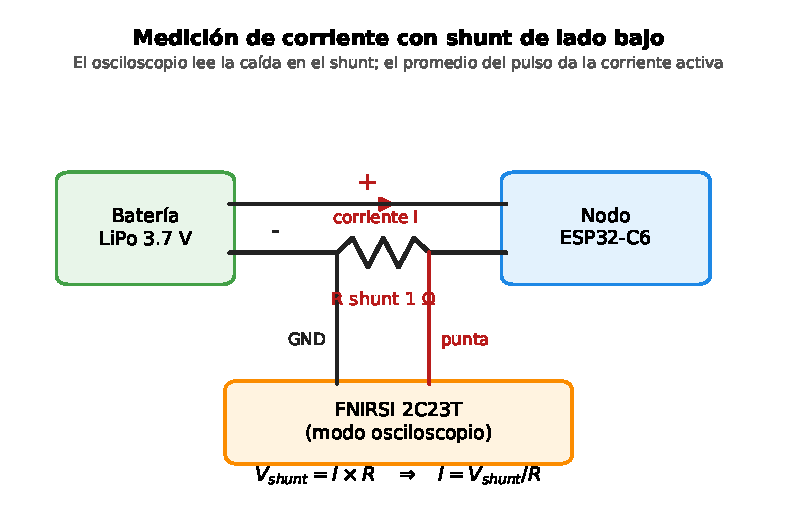
\includegraphics[width=0.60\textwidth]{montaje-corriente.pdf}
\caption[Montaje propuesto para medición de corriente con shunt.]{Montaje documentado para medir corriente a partir de la caída en un shunt de lado bajo. Explica la conexión y conversión tensión--corriente; no acredita una captura experimental del pulso ni la corriente total de sueño. Fuente: diagrama del repositorio.}
\label{fig:metodo-montaje-corriente}
\end{figure}

\section{Trazabilidad y límites de reproducción}
Reproducir el análisis requiere CSV, fechas, MAC, configuración y registros serie de los ensayos. Varios scripts usan rutas personales; su publicación no aporta los datos ausentes. Cada resultado debe distinguir medición, transformación y estimación.

\chapter{Desarrollo e implementación}
Este capítulo documenta la construcción de los nodos, el gateway, el almacenamiento y el dashboard local.

\chapter{Resultados y evidencias}
Este capítulo presenta las evidencias de funcionamiento, comunicación y operación energética obtenidas en la evaluación.

\chapter{Discusión, limitaciones y amenazas a la validez}
Este capítulo interpreta los resultados y expone las limitaciones de la evidencia disponible.

\chapter{Conclusiones y trabajo futuro}
Este capítulo presenta las conclusiones vinculadas con los objetivos y las líneas de trabajo futuro.

\bibliographystyle{apalike}
\bibliography{tesis/referencias}
\clearpage
\appendix
\chapter{Información complementaria y reproducibilidad}
Este anexo reúne información complementaria para reproducir los cálculos, las pruebas y los artefactos del proyecto.

\end{document}
